\documentclass[a4paper,12bp]{report}
%Packages Import
\usepackage[utf8]{inputenc}
\usepackage[pdftex]{graphicx}
\usepackage{algpseudocode}
\usepackage{algorithm}
\usepackage{mathtools}
\usepackage{url}
\usepackage{enumerate}
\usepackage{verbatim}
\usepackage{diagbox}
\usepackage{eucal}
\usepackage{lipsum}
\usepackage{titlesec}
\usepackage{amsfonts}
\usepackage{amsthm}
\usepackage[left=1.5cm,right=1.5cm,top=3cm,bottom=3cm]{geometry}
\usepackage{multirow}
\usepackage{subcaption}
\usepackage{listings}
\usepackage{xcolor}
\usepackage{indentfirst}
\usepackage{setspace}
\usepackage{textcomp}
\usepackage{tocloft}
\usepackage{enumitem}
\usepackage{lmodern}
\usepackage{array}
\usepackage{times}
\usepackage{appendix}

% Avoid widows and orphans
\widowpenalty10000
\clubpenalty10000

% New Commands
\newcommand{\lbr}{\ensuremath{\left\lbrace}}
\newcommand{\rbr}{\ensuremath{\right\rbrace}}
\newcommand{\mcl}[1]{\ensuremath{\mathcal{#1}}}
\newcommand{\method}[2]{\ensuremath{\text{#1} \left( #2 \right)}}
\newcommand{\ttm}
{\ensuremath{^{\text{\texttrademark}}}\enskip}
\newcommand{\tcr}
{\ensuremath{^{\text{\textcopyright}}}\enskip}
\newcommand{\treg}
{\ensuremath{^{\text{\textregistered}}}\enskip}

\newcommand{\incode}[1]{\texttt{#1}}
\newtheorem{definition}{Definition}
\newtheorem{theorem}{Theorem}

% Format Titles and Sections
\titleformat{\chapter}[display]
{\centering\bfseries\fontsize{18pt}{20pt}\selectfont}{\chaptertitlename \hspace{2mm} \thechapter}
{5mm}{}

\titleformat{\section}
{\bfseries\fontsize{16pt}{18pt}\selectfont}
{ \thesection\hspace{2mm}}
{1mm} {}

\titleformat{\subsection}
{\bfseries\fontsize{14pt}{16pt}\selectfont}
{ \hspace{2mm} \thesubsection}
{1mm} {}

\titleformat{\subsubsection}
{\bfseries\fontsize{13pt}{13pt}\selectfont}
{ \hspace{2mm} \thesubsubsection}
{1mm} {}


\setlength{\parindent}{12mm}
\setlength{\parskip}{2.5\baselineskip}


\titlespacing*{\chapter}{0pt}{55mm}{15mm}
\titlespacing*{\section}{0pt}{1mm}{1mm}
\titlespacing*{\subsection}{0pt}{1mm}{1mm}


\begin{document}

% Title Sheet
\begin{titlepage}
 
 \begin{center}
  \huge\textbf{Stock Market Prediction Model using Financial News Documents}
  
  \vspace{5mm}
  \large Submitted in the partial fulfillment for the requirements of the 
degree of\\
\Large\textbf{Master of Technology}\\
\large in\\
\Large\textbf{Computer Science and Engineering}\\
\vspace{15mm}
\Large By\\
\vspace{3mm}
\Large\textbf{Saurav Das\\
Roll: 127521}\\
\vspace{15mm}
\Large Supervisor:\\
\vspace{3mm}
\Large\textbf{Prof. S.G.Sanjeevi}

\vspace{10mm}

\includegraphics[scale=1]{pictures/nitw-logo.png}

\vspace{5mm}
\large \textbf{DEPARTMENT OF COMPUTER SCIENCE AND ENGINEERING\\
NATIONAL INSTITUTE OF TECHNOLOGY\\ WARANGAL - 506 004\\
2013--2014}
 \end{center}

\end{titlepage}
% Title Sheet End

\pagenumbering{roman}

% Approval Sheet
\newpage
\thispagestyle{empty}
\begin{center}
\LARGE{\textbf{Dissertation Approval for M.Tech}}
\end{center}

\Large {
This Project Work entitled ``Stock Market Prediction Model using Financial News Documents''  by Saurav Das is approved for the Degree of M. Tech in Computer Science and Engineering.
\begin{center}
Examiners:\\
\underline{\hspace{6cm}}\\
\vspace{5mm}
\underline{\hspace{6cm}}\\
\vspace{5mm}
\underline{\hspace{6cm}}\\

\vspace{15mm}
Superviser(s):\\
\underline{\hspace{6cm}}\\
\vspace{5mm}
\underline{\hspace{6cm}}\\
\vspace{5mm}
\underline{\hspace{6cm}}\\
\vspace{15mm}
Chairman:\\
\underline{\hspace{6cm}}\\
\end{center}
\vspace{15mm}
Date: \underline{\hspace{6cm}}\\
\\ 
Place:\underline{\hspace{6cm}}\\
}
% Approval Sheet End

% Certificate
\newpage
\begin{center}
\Large{\textbf{DEPARTMENT OF COMPUTER SCIENCE AND ENGINEERING\\
NATIONAL INSTITUTE OF TECHNOLOGY,\\
WARANGAL - 506 004}}

\vspace{10mm}

\includegraphics[scale=1]{pictures/nitw-logo.png}

\vspace{10mm}
\underline{CERTIFICATE}
\end{center}
\Large {
This is to certify that the project titled ``Stock Market Prediction Model using Financial News Documents'' is a bonafide work carried out by Saurav Das in partial fulfillment of the requirements for the award of the degree of M.Tech (Computer Science and Engineering) and submitted to the Department of Computer Science and Engineering, National Institute of Technology, Warangal.

\vspace{10mm}
\noindent Prof. S.G.Sanjeevi \hfill Dr. K. Ramesh\\
\noindent Project Guide \hfill Head of the Department
}

% Certrificate End

\newpage

%Academic Honesty
\large {
\begin{flushleft}
Department of CSE,\\
NIT, Warangal - 506004
\end{flushleft}
\begin{center}
\LARGE{\textbf{Declaration of Academic Honesty}}
\end{center}
\Large
I declare that this written submission represents my ideas in my own words and where others' ideas or words have been included, I have adequately cited and referenced the original sources. I also declare that I have adhered to all principles of academic honesty and integrity and have not misrepresented or fabricated or falsified any idea / data / fact / source in my submission. I understand that any violation of the above will be cause for disciplinary action by the Institute and can also evoke penal action from the sources which have thus not been properly cited or from whom proper permission has not been taken when needed.
\vspace{2cm}

\underline{\hspace{6cm}}

(Signature)

\vspace{2.5mm}
Saurav Das

\vspace{2.5mm}
(Roll: 127521)

\vspace{2.5mm}
Date: \underline{\hspace{6cm}}
}
% Academic Honesty End


\begin{doublespacing}

\begin{abstract}
\setcounter{page}{4}
Stock market prediction based on financial news has been studied previously by many researchers. We examine that the changing news in the market and the concept-drift in the market can affect the static feature space prediction methods. So, we take a dynamic feature space to correctly represent the changing concepts and their effects in the market. We design a prediction model that uses the changing feature space, classifies the new news articles and then uses an Artificial Neural Network to predict the BSE S\&P 500 Sensex index. A profitable intra-day trading system is developed to get us better returns for trader investment. 

\textbf{Keywords} : Text Mining, Financial Prediction, News Classification.
\end{abstract}
\end{doublespacing}
\newpage
\setcounter{page}{5}
\setlength{\cftbeforechapskip}{1em}
\setlength{\cftbeforesecskip}{0.5em}
\setlength{\cftbeforesubsecskip}{0.5em}
\setlength{\cftbeforefigskip}{0.5em}
\setlength{\cftbeforetabskip}{0.5em}
\renewcommand{\cfttoctitlefont}{\LARGE\bfseries}
\renewcommand{\cftloftitlefont}{\LARGE\bfseries}
\renewcommand{\cftlottitlefont}{\LARGE\bfseries}

\tableofcontents
\newpage
\listoffigures
\newpage
\listoftables

\doublespacing
\newpage
\pagenumbering{arabic}
\chapter{Introduction}
\label{chap:introduction}
\thispagestyle{empty}

Stock market has been a field of interest for businessmen, common people and researchers as well for many years. Several methods has been adopted and designed for predicting the stock market values. These predictions help traders make better decisions regarding the trading of stocks. News coverage by the media carries much information regarding the current trends of a market. For each development the on-line news stream provides live coverage. This news motivates or gets people away from stocks of particular kind. Thus news articles have a wide potential in changing the market. So it can be used to determine the trend in the market. This has been the basic theory by several researchers who have predicted trends in the market according to the recent news developments.

Since the advent of Internet and strong networking, there is a large content of data in the form of news available. There are news articles, on-line blogs by stock gurus and company notifications which provides loads of information about the market. The market today is guided by several different kinds of news from several sources. Now stock traders use these sources to make trading decisions and this affects the market. So, an automated system which can predict the change in market due to some news would give us the same effect as an experienced stock trader.

Text mining methods are used to classify news and predict news sentiments. However popular methods have already found out that the sentiment of an article is not of main relevance here. In a particular context some article which may contain negative words may also have reason to cause stock market to rise. So normal classification techniques can't be used, and modified techniques should be used to evaluate the news articles.

The stock market has always been heavily affected by breaking news releases since they drive the people for making rapid market decisions. There is loads of information available on-line in the form of Natural Language Text. The dream is to design proper techniques to be used so that machines can analyse these news and make marketing decisions automatically.

Existing research regarding this field has developed ways to mine the content in the news articles and formulate effective methods of trading according to the news. Hagneau et al. in \cite{Hagenau:2013} has formulated good feature extraction techniques which give much more representative features to represent documents. The AZFinText model developed by Schumaker et al. in \cite{Schumaker:2009} is also an important model used for predictions.

Our motivation for the research was based on capturing the change in the underlying concept, and how news features keep changing with time and in case of financial market the most recent news may contain some trend capturing context which was previously not there during the training phase of the models. So a dynamic training with feature set up-gradation is necessary for the effective understanding of the underlying semantics of news articles. We design a prediction model that uses the changing feature space, classifies the new news articles and then uses an Artificial Neural Network to predict the BSE S\&P 500 Sensex index. A profitable intra-day trading system is developed to get us better returns for trader investment. 

\section{Objectives}
The main objective of this thesis is to design a stock market prediction model which will give us better intraday trading. Traders can use this model to get better benefit for their investment in the market. This prediction model predicts the trends by analyzing the current news on the market and considering how those news affects the market. The news documents are classified as to what effect they'll have on the market. A dynamic feature space approach with projected clustering method has been taken to classify the news documents properly. 

\section{Organization of the Thesis}

The rest of the thesis has been organized in several chapters. In chapter 2, we discuss some of the theories regarding stock market predictions and the different existing researches in this field. A brief description of the methodologies adopted by them is described in this chapter. In chapter 3, we talk about the questions which drive this research and the approaches used by the model designed by us. The different theories which help us design the model has been provided here. In chapter 4, the details regarding the actual implementation of our model has been discussed. We discuss in detail how the different  modules has been designed and their working. In chapter 5, experiments are set-up to verify the working of our prediction model on real data set. In chapter 6, our approach is summarized and future ways to develop the model has been talked about. 

\chapter{Literature Survey}

There has been a lot of work in the field of stock market prediction. There are two prevalent theories that are related to the market predictions. The Efficient Market Hypothesis (EMH) and the Random Walk Theory (RWT).

In finance, the Efficient Market Hypothesis (EMH), or the Joint Hypothesis problem, asserts that financial markets are "informationally efficient". In consequence of this, one cannot consistently achieve returns in excess of average market returns on a risk-adjusted basis, given the information is available at the time the investment is made \cite{ wiki:20141}. There are 3 forms in which the EMH theory is represented as - weak-form efficiency, strong-form efficiency and semi-strong-form efficiency. In weak-form efficiency we cannot detect future prices by seeing the past trends. In semi-strong-form efficiency share prices are adjusted easily when new information about the share comes to product, thus making share prices change in a very quick and unpredictable fashion. Strong-form efficiency states that since every foreseen change is public therefore no extra gain can be obtained from the market. 

The random walk hypothesis is a financial theory stating that stock market prices evolve according to a random walk and thus cannot be predicted \cite{ wiki:20142}. The Random Walk Theory is also consistent with the Efficient Market Hypothesis. 

So, according to the two hypothesis it is very difficult to predict trends in the future stock market, making it a problem. It is not possible to accurately predict the market behaviour at all times because ultimately the driving force of stock market is the traders. When more trade of stocks is there stock market is in a bull else it is a bear market. 

Though the Efficient Market Hypothesis and Random Walk Theory say that stock values cannot be predicted, researchers do not agree to this theory completely. Several counter theories and models have been designed which has been seen to provide considerable amount of gain in the market. The semi-strong-form efficiency of the market is used along with the rapid analysis of information to give hint as to which direction the market is going. Machine learning techniques help in this process. 

Our project is mainly concerned about the change in the stock market index. The prediction of stock market index with financial news as aid, which gives us hints about which way the stock market is being driven to. 

The Bombay Stock Exchange (BSE) is a stock exchange in Mumbai, India. It is the 11th largest stock exchange in the world in terms of Market Capitalization \cite{ bse:20}. The popular index of BSE is the S\&P BSE SENSEX. It is the most tracked benchmark index in India. It is traded internationally on the EUREX as well as leading exchanges of the BRCS nations (Brazil, Russia, China and South Africa). On Tuesday, 19 February 2013 BSE has entered into Strategic Partnership with S\&P DOW JONES INDICES and the SENSEX has been renamed as "S\&P BSE SENSEX" \cite{ wiki:20143}.

The basic strategy of news based trading is to buy or sell stocks according to the market news. But this is not applicable always, because sometimes the news in the market is already anticipated so even a good news does not have that much difference in the stock market prices as the effect is slowly dissolved in the market and the market has adjusted itself in anticipation. Best changes are found out due to the breaking news which cause the drop or rise in market values. 

Stock trading has been affected due to economic news publications \cite{RePEc:eee:pacfin:v:9:y:2001:i:3:p:195-217}. However not always can the financial news correctly predict the market changes, because other factors are still relevant in the market. There are also sudden unforeseen rise and fall of prices in the market because of large amount of trades \cite{camerer1991information}. 

Many researchers have worked on this concept and many different models have been designed which deal with time series stock market prediction. The data set which has been used in prediction comprises of the financial message base and the stock market change after this news item is released. The financial message base may contain financial news articles as used in \cite{Schumaker:2009}\cite{JOFI:JOFI1362}\cite{1265201}, ad-hoc corporate announcements as used in \cite{conf/wirtschaftsinformatik/GrothM09}\cite{groth2011intraday}, worldwide general news as used in \cite{725072}, corporate filings as used in \cite{JOAR:JOAR382}, message postings as used in \cite{doi:10.1287/mnsc.1070.0704} or annual reports as in \cite{butler:2009}.

The financial news obtained have to correctly processed and represented in a format which can help machine learning algorithms properly analyse the data and train accordingly. Text mining on the news body is done for feature processing. Feature processing comprises of 3 steps -
\begin{enumerate}
\item Feature Extraction

In this step the type of features which are used to represent the documents are defined. Features are extracted accordingly which best reflect the content of the documents. Many different approaches of feature extraction has been used by different researchers such as bag-of-words \cite{conf/wirtschaftsinformatik/GrothM09}\cite{1265201}\cite{725072}\cite{JOAR:JOAR382}\cite{antweiler2004all}, noun phrases \cite{Schumaker:2009}, n-grams \cite{butler:2009}, 2-word combinations \cite{Hagenau:2013}. 

\newpage
\item Feature Selection

In the feature extraction step many features are generated which are not all important and maximum of them comprise of redundant features. We need to take a subset of the features extracted which will give us the best features to represent the documents. Different feature selection methods used are - Dictionary based \cite{JOFI:JOFI1362} and Exogenous market feedback \cite{groth2011intraday}\cite{Hagenau:2013}. Chi-Square and Bi-Normal Separation are some of the statistical methods which are used for the selection process.

\item Feature Representation

Documents need to be represented in machine readable format so that machine learning algorithms can be applied on them. Feature representation is the step of converting the documents to machine readable format so that learning algorithms can train themselves on these document vectors and make future predictions. 
\end{enumerate}
After the feature processing is completed and the documents of the data set are converted in machine readable format machine learning algorithms are applied on them. The stock market prediction is concerned with predicting the trend of the market. This is achieved by training the machine using various algorithms. Many different algorithms have been used by the researchers. Support Vector Machine (SVM) is a very popular method in \cite{Schumaker:2009}\cite{conf/wirtschaftsinformatik/GrothM09}\cite{1265201}. Na\"{i}ve Bayes has been used in \cite{725072}. A combination of Bayes and SVM has been used in \cite{antweiler2004all}, Ratio of negative words has been used in \cite{JOFI:JOFI1362}. Propriety distance measures has been used in \cite{butler:2009}. The classification accuracy is the main metric which is examined to determine how well the news is being classified. 

We will discuss some of the popular existing architectures which deal with news based stock market prediction.
\newpage
\begin{enumerate} 
\item \textbf{NewsCATS}

The NewsCATS method was designed by Mittermayer \cite{1265201}. It tries to predict price trends immediately after the publication of a news item. The architecture of the NewsCAT system comprises of mainly 3 steps.

\begin{enumerate}
\item Document Pre-processing Engine

This component retrieves information from press releases and then pre-processing steps are applied on them like tokenizing, stop-word removal and stemming. Bag of words is used as the feature selection process, selecting 1000 words having the maximum WDFxIDF score. 

\item Categorization Engine

Each news is categorized into 3 different classes. They are - 'Good news', 'bad news' and 'neutral news'. Support Vector Machine is used for the classification.

\item Trading Engine

30 seconds after news publication positions were opened for stock trading. Profits are taken immediately if the value of investment rises more than 1\% or more. In case of loss, a two-sided early exit strategy is applied. 0.5\% for gains and stop loss transactions if the position falls below -2\%. 
\end{enumerate}

\item \textbf{AZFinText}

The AZFinText mode was designed by Schumaker \& Chen \cite{Schumaker:2009}. It also considers financial news for prediction of stock movements. The architecture comprises of -

\begin{enumerate}
\item Feature selection and representation

In the AZFinText model proper nouns are extracted as features and proper nouns that occur 3 times or more are included in the feature set. Along with features the overall tone of the article is also considered. The OpinionFinder tool is used to mark the article whether it is more objective or subjective. 

\item Prediction Engine 

Support Vector Regression mechanism is used for the prediction of actual stock prices. A 20 minute later stock price is predicted by the model. 

\item Trading Engine

The trading engine used is a modified version of Lavrenko's Trading Engine \cite{lavrenko2000language} which examines the return percentage of a stock. When a predicted movement of 1\% is noted in the stocks then \$1000 worth of the stock is bought or short-selled and then disposed off in the next 20 minutes. 
\end{enumerate}

\item \textbf{Method proposed by Hagneau}

The method used has been designed by Hagneau et al. \cite{Hagenau:2013}. It is of the same domain as the other two methods and gives the best accuracy among all the previous methods designed by researchers. The architecture is composed of - 
\begin{enumerate}
\item Features extraction \& selection 

The features module is used to extract features from the natural language documents and select the features which are most relevant. Hagneau et al. first introduced a new kind of feature called \textit{Word Combinations} which has a better capability to capture the semantics of the documents. All word combination features are extracted from the documents and \textit{Bi-Normal Separation} technique is used to select the relevant features among them. 

\item Classification of news articles

A Support Vector Machine (SVM) is used to train according to the past news document vectors and the sentiments marked according to the exogenous market feedback. The SVM is used to classify the new news articles.

\end{enumerate}
\end{enumerate}

These are some of the existing popular architectures in the intra-day stock market prediction field. They have used popular text mining methods and machine learning techniques in their models to use the news content for prediction purposes. In the following chapter we talk about the problem figured in the existing methods and our approach to design a better prediction system. 

\chapter{Stock market prediction model design}

The Related work shows us about the various approaches used by researchers in trying to predict the stock price and ultimately developing a trading system to maximize profit from stock market. In this chapter we define the research goals and objectives of our project finding scope for improvement in the related work. 

\section{Research Questions}
For our research there are 3 major questions which we will be using to find a better model or prediction strategy. Our project mainly focuses on the problems with the current processes and their probable solutions. The Questions are - 
\begin{enumerate}
\item \textbf{Question} : Does a fixed feature space capture all trends of the stock market?

The work done by the previous researchers all comprise of fixed feature space models. The classification or regression models used by the researchers all have a static feature space and when some new item comes those specific features are searched and the new item is classified accordingly. The concept drift in the data is not considered in these methods.In machine learning, the concept drift means that the statistical properties of the target variable, which the model is trying to predict, change over time in unforeseen ways. This causes problems because the predictions become less accurate as time passes \cite{ wiki:20146}. 

We are trying to predict stock market by using context capturing features from the financial news items. As far as news is considered, the determining factors in a news in ever changing. There are always new buzzwords in the market which are determinants of the stock market. For a financial market, a company when is on loss can fall under negative  determinant while if the same company sees boost in market, perhaps due to some acquisition then the company can be considered as a positive determinant for the market. 

A fixed feature space won't be able to capture these recent trends in the stock market, because it's features will always be limited to the trends predominant in the time the machine learning model was trained. And if the model is trained according to news data which are widely spanned, then they will capture the most generalized trends of the market. However market determinants are generally not the generalized terms but those which are the recent trend-setters affecting the market. Since we are concerned about intra-day predictions thus features helping in short changes in market can be helpful. So instead of a fixed feature space, a  dynamic feature space may help us consider better context capturing features. 

\item \textbf{Question} : How little can training phase be for the prediction of stock data?

Generally extensive training of prediction models are done before the model is actually used for the prediction purpose. But is extensive training always effective and necessary? Extensive training may lead to over-fitting of training to the data. And training according to some very old data will only give us old trends. Old trends however are not relevant in the current time frame. So it's rather unnecessary to train for all the data when only the most recent data will determine the changes. In the stock market always there are new trends and price changes vary with time. So, extensive training over a large period of time may cause more generalization rather than capturing the trend specific to the present time. 

\item \textbf{Question} : Can a trading strategy be defined by using the Index value?

The previous researches have all developed a trading strategy based on the prediction of the stock price of a specific stock. However in this research we formulate a new trading system where the trades occur according to the S\&P BSE Sensex Index. The BSE index correctly reflects the current market conditions. The index is calculated based on a free float capitalization method, a variation of the market capitalization method. Instead of using a company's outstanding shares it uses its float, or shares that are readily available for trading \cite{ wiki:20144}. In short term intra-day trading thus the market index can help better understand the total market situation instead of a single stock situation and can help foresee situations. In stock market chaining effects take place which means that the effect in one stock can cause simultaneous in other stocks of related field. So, an overall effect analysis may possibly cause better trading and increased returns. 
\end{enumerate}

\section{Solutions proposed}
\begin{enumerate}
\item \textbf{Problem} : Fixed feature space doesn't capture recent trends

\textbf{Solution} : 

The problem with a fixed feature space has already been discussed in our research questions where it's evident that the problem with static feature space is that recent features are not captured by the classifier. Thus a dynamic feature space would be much better in this case. The conversion of a static feature space to a dynamic feature space is done according to the lossless homogeneous feature space conversion. We will discuss about the lossless homogeneous feature space conversion in the subsequent sections. The new documents are classified by clustering of the points. However, the dynamic feature space conversion increases the feature space size considerably and thus dimensionality of the document vectors also increases. This causes a problem as it is difficult to classify high dimensional data points because they tend to become equidistant from each other. The distance to the nearest data point is similar to the distance to the furthest point \cite{Beyer:1999} and this can be attributed to the 'curse of dimensionality'. 

\item \textbf{Problem} : For high dimensional data due to sparsity of data points, all points tend to become equidistant from each other.

\textbf{Solution} : 

The problem faced by the feature space conversion is that it causes the points in the feature space to become equidistant from each other. The high dimensional feature space prevents proper clustering of data points due to the sparsity of data points. This can be solved by using methods like - subspace clustering or projected clustering. We use projected clustering because of it's quick computation and less management of different subspaces. In this method, some points are correlated with one set of dimensions while other points are correlated with a different set of dimensions \cite{Aggarwal:1999}.
\end{enumerate}

\section{Approach Overview}
The approach used in the project is briefly defined here. The main training base for our project are the financial news articles. News articles are classified into 3 classes - 'positive', 'negative' and 'neutral'. The 'positive' class defines those articles that will boost the stock market, the 'negative' class contains articles which will cause a downfall of stock prices and the 'neutral' class does not cause much change to the stock market.

Our project mainly comprises of 2 phases -

\begin{enumerate}
\item \textbf{ANN training phase}

In this phase data is collected for training of the Artificial Neural Network (ANN) model which is used later for the prediction of the stock price. The ANN model takes in the change in the stock market index in the previous 15 minute time frame along with other financial parameters and news sentiments and then predicts the change in the next 15 minutes.

\item \textbf{Market Prediction phase}

For our model the only pre-training is done on the previous data. The features which would form the feature space for classification are chosen dynamically. Initially a feature space is defined using the news items from the previous day. The news items from the previous trading day form the initial clusters. Any new news which comes is classified using projected clustering. After the news at a particular time is classified into a particular sentiment class it is fed into the ANN along with other factors as a parameter to determine the movement of the stock index.
\end{enumerate}

\section{Data Acquisition}
For our prediction purpose we need financial news and stock market data. These data has been collected from the web. The financial news articles are labelled according to the exogenous market feedback as done in \cite{Hagenau:2013}. This method has been proved to be better because it gives us the most relevant features differentiating between the different classes of news. For our data acquisition phase we also need data about certain other determinant factors which will affect the stock market. The change in values of these factors too need to be collected so that they can be used to train our Artificial Neural Network which will predict the stock index value. 

\subsection{Collection of news articles}
The news articles are used to predict the stock market sentiment. The news articles are primarily of financial domain, which would give us the best overview about the current stock market. Stock prices are collected along with the news articles and then according to the stock price change after the news article is released, the news article is labelled as positive, negative or neutral. The news articles considered are breaking news released at frequent intervals by the media or stock analysts. 

\subsection{Collection of Stock Quotes}
The stock quotes are collected alongside the news articles to determine the change in stock movement. This helps in labelling the news articles and acts as a parameter in the Artificial Neural Network.

\subsection{Collection of other parameters}
\label{sec:ann_parameters}
There are other parameters which are considered when predicting the stock price movements. These economical parameters are very important for the stock market. The following factors are primarily considered as parameters affecting the Indian market according to \cite{ghosh:2010}. They are - Crude Oil price, Gold price, Cash Reserve Ratio, Food price inflation, Call money rate, Dollar price, FDI, Foreign Portfolio Investment and Foreign Exchange Reserve (Forex). Since we are predicting the intra-day stock price changes we consider those components whose values change intra-day. The Cash Reserve Ratio, Food price inflation, Call money rate, FDI, Foreign Portfolio Investment and Foreign Exchange Reserve (Forex) are economic determinants but they change quarterly or monthly. So, they are not considered for our project. Only Crude Oil price, Gold price, Dollar Exchange rate changes are considered for market prediction. 

\section{News Labelling by stock price}
The financial news collected is labelled according to the financial news. The different classes are - positive, negative and neutral. 

We devise a method for determining the label of a news article. As the news articles is released the stock price change is noted every 5 minutes. A total of 15 minutes time window is kept for the news affecting the stock market. The 15 minute window is divided into 5 minute intervals. 50\% importance is given to the change in the first 5 minutes. 30\% importance to the second 5 minutes and 20\% importance is given to the last 5 minutes.
\begin{equation}
change_{total} = ( bsechange_{1} ) \times 0.5 + ( bsechange_{2} ) \times 0.3 + ( bsechange_{3} ) \times 0.2
\end{equation}
$change_{total}$ : Total change in the 15 minute window \\*
$bsechange_{1}$ : The change in the first 5 minutes \\*
$bsechange_{2}$ : The change in the second 5 minutes \\*
$bsechange_{3}$ : The change in the last 5 minutes \\*

This gives maximum importance to the change in the first minutes and gradual decrease in the change importance. The labelling of the documents is done as follows - 

\begin{equation}
sentiment=
	\begin{cases}
		positive, & \text{if}\ change_{total} \geq change_{threshold} \\
		negative, & \text{if}\ change_{total} < 0.0 \\
     	neutral, & \text{otherwise}
	\end{cases}
\end{equation}

The $change_{threshold}$ is taken as 5.0. News articles which cause more than 50\% increase or decrease in the values of stock are considered as positive or negative news respectively. The other news items are however considered as neutral, making minimum changes which are inherent in stock markets and can't be really attributed to some change caused due to news. 

\section{Preparation of News articles}
After the news articles have been gathered by our collector and before the news article is used for classification prediction or classifier training the news article needs to be pre-processed properly and made ready for the machine learning algorithm to be applied on it. 

The various steps required for the preparation of the news articles are - \\* 
(1) Document Pre-processing \\*
(2) Feature Extraction \\*
(3) Feature Selection \\*
(4) Document Representation

\subsection{Document Pre-processing}
\label{subsec:pre-processing}
The document pre-processing consists of the following steps - 
\begin{enumerate}
\item \textbf{Removing punctuation marks}

All punctuation marks are removed from the news text body. All numbers and symbols are also removed. Only plain text is kept as the news body. 

\item \textbf{Tokenizing}

The text is broken down into tokens of words separating the words by the white spaces. 

\item \textbf{Stop-word removal}

Stop words are the words which are found most frequently in text and they do not really add anything to the content. They are there for providing structure in the sentence. Thus the stop words are mainly removed before text processing is done on any natural language articles. 

\item \textbf{Stemming}

Stemming is the process of converting the words in text into a single form. Same words in text documents can be in different forms. These words have same meaning but they differ in the way they are represented. Thus a stemming algorithm is generally used which converts words with the stems to their root form thus making different words similar. The Porter Stemmer algorithm \cite{porter1980algorithm} is a very popular stemming algorithm and has been used in our project.
\end{enumerate}

\subsection{Feature Extraction}
We need to extract features from the news documents which will define the documents properly. These features will help us determine the document class. The feature type that we use in our project is 2-word combinations. This has been used in \cite{Hagenau:2013}.

2-words combination is an extension of the 2-gram feature type. In 2-grams the word distance between two words is zero. However in the case of 2-word combinations the distance between two words may be more than zero. More possible combination of features are found by this method, and it also helps capture better features because not only neighbouring words grouped together have meanings but also two words in a sentence grouped together may also carry important meaning. 

\subsection{Feature Selection}
The feature selection is the method of selecting only the features which are most effective in creating differentiating two documents. Feature extraction gives us many features by providing all combination of words found in the news documents. Among these features the few features which have high explanatory power are taken as the features for representing documents. 

The explanatory power of the features are determined by the statistical method of Bi-Normal-Separation (BNS). The BNS method is chosen as it has been found best performing in \cite{Hagenau:2013}. The BNS selection method determines the prevalence of a feature in a specific class rather than in the rest classes. The features which give the maximum difference is taken as the differentiating feature, because they will help effectively to classify the documents. The BNS formula we use is defined as - 
\begin{equation}
\label{eq:bns}
BNS_{i} = max \left\{ F^{-1} \left(\frac{O_{i,x}}{|x|}\right) - \sum_{y \in \{S - x\}} F^{-1} \left(\frac{O_{i,y}}{|y|}\right)  \middle| x \in S \right\}
\end{equation}
where, $S = \{ positive, negative, neutral \}$ are the different sentiment classes. $F^{-1}$ is the standard normal distribution's inverse normal cumulative probability function or z-score. $O_{i,x}$ denotes the observed frequency of the number of instances of the occurrence of feature $i$ in the class x documents. The value of $F^{-1}(0)$ is substituted by 0.0005 \cite{Forman:2003}.

\subsection{Document Representation}
After the feature selection is done we get a feature space. This feature space is used to create the document vectors as in Vector Space Model. The Vector Space is an algebraic model for representing documents as vectors of identifiers \cite{ wiki:20145}. A particular document $D_{j}$ is represented as - 
\begin{equation}
d_{j} = ( w_{1,j} , w_{2,j} , ... , w_{n,j} )
\end{equation}
where, $w_{i,j}$ is the weight of feature $i$ in document $j$. $n$ is the total number of features present in the feature space. 


The document vectors give us the weights of the different features in the feature space for the document. The length of each of the document vectors is equal to the length of the feature space. The features which are not present in the document are given zero weight-age. The weight metric selected for our project is TF-IDF measure. The Term frequency-Inverse Document Frequency is a statistic measure which reflects the importance of a term for a document.

The term frequency $tf(t,d)$ is simply the number of times the term $t$ occurs in the document $d$. The augmented frequency $tf$ value is taken as it prevents bias towards longer documents. The raw frequency is divided by the maximum frequency of any term in the document. The value of $tf(t,d)$ is calculated as -
\begin{equation}
tf(t,d) = 0.5 + \frac{0.5 \times f(t,d)}{max\{ f(w,d) : w \in d \}}
\end{equation}
where $f(t,d)$ is the frequency of the term $t$ in the document $d$. 

The Inverse Document Frequency (IDF) is a measure of how frequently the word occurs in the documents. Whether the term is rare or frequent among documents. The value of $idf(t,D)$ is calculated as - 
\begin{equation} 
idf(t,D) = log \frac{N}{1 + |d \in D : t \in d|}
\end{equation}
where, N is the total number of documents in the corpus and $|d \in D : t \in d|$ is the number of documents where term $t$ is present. 

Then TF-IDF is calculated as -
\begin{equation} 
\label{eq:tfidf}
tfidf(t,d,D) = tf(t,d) \times idf(t,D)
\end{equation}

\section{Lossless Homogeneous Feature Space Conversion}
\label{sec:lhfs}

Every time we come across a new news document we collect new features from the document. In our project a dynamical feature space is being considered to deal with the problem of capturing the recent stock market buzzwords. We extract the features that are most discussed in the recent news documents. Lossless Homogeneous feature space conversion has been used to change the feature space in \cite{Masud:2010}. Each time we select 40 new features to add to the existing feature space. We use a modified version of the feature space conversion technique to suit our needs better. 

The steps for the feature space conversion are as follows - 
\begin{enumerate}
\item A block of the most recent news articles are kept containing the last 10 news articles released before the release of the present news article. From this block of news articles we extract and select the best 1000 features according to the 2-word combinations and Bi-normal-separation techniques respectively.

\item From the new news documents we extract all the 2-word combinations as features.

\item The features set we got from the new news articles and the feature set selected from the most recent news articles are intersected to form a set of features. 60\% of the extended feature set are added from this intersection set. 

\item The features in the new articles which are completely new, not present previously in any news articles form a new set of features. These features are ranked according to the frequency of their occurrence in the news articles. The most frequent features make up the rest 40\% of the extended feature set. 
\end{enumerate}

\section{Fading Cluster}
\label{sec:fading}
The news data stream which we have consists of multiple data points in a time stream. The Fading Clusters concept for handling data points in a data stream has been introduced in \cite{Aggarwal:2005} to provide more importance to the most recent data points. In time stream data recent data points capture the most recent trends and thus should be given more value than the older points in the stream. The fading cluster data structure contains the information about the data points present in the cluster. Each data point has a weight assigned to it according to the fading function $f(t)$ whose value lies between (0,1). The fading function is a monotonically decreasing exponential function which decays uniformly with time $t$. The fading function $f(t)$ is defined as- 
\begin{equation}
f(t) = 2^{-\lambda \cdot t}
\end{equation}
where, $\lambda$ is the decay-rate and is defined as the inverse of the half-life of the data stream and t is the time at which the data point came to the data stream. Thus, $\lambda = 1/t_{0}$, $t_{0}$ being the half-life time for data points. According to the formula for the fading function $f(t)$ a gradual exponential decay of the data points takes place. This satisfies the property of giving maximum weight-age to the most recent data items rather than the old ones.

The definition of the fading cluster structure as given by Charu et al. in \cite{Aggarwal:2005} is given as - 
\newtheorem{mydef}{Definition}
\begin{mydef}
A fading cluster structure at time t for a set of d-dimensional points $C = \{X_{i_{1}}, ..., X_{i_{n}}\}$ with time stamps $T_{i_{1}}, ... , T_{i_{n}}$ is defined as the $(2 \cdot d + 1)$ tuple $FC(C,t) = (\overline{FC2^{x}(C,t)}, \overline{FC1^{x}(C,t)}, W(t))$. The vectors $\overline{FC2^{x}(C,t)}$ and $\overline{FC1^{x}(C,t)}$ each contain d entries. 
\end{mydef}

The different parts of the Fading Cluster structure are defined as - 
\begin{enumerate}
\item For each dimension $j$, the $j$-th entry of $\overline{FC2^{x}(C,t)}$ is the weighted sum of the squares of the corresponding data values. This defines a time-decaying second order moment of the data points. $\overline{FC2^{x}(C,t)}$ contains d values, for each dimension. The $j$-th entry of $\overline{FC2^{x}(C,t)}$ is given as $\sum_{k=1}^{n} f(t-T_{i_{k}}) \cdot (x_{i_{k}}^{j})^2$

\item For each dimension $j$, the $j$-th entry of $\overline{FC1^{x}(C,t)}$ is the weighted sum of the corresponding data values. This defines a time-decaying first order moment of the data points. $\overline{FC2^{x}(C,t)}$ contains d values, for each dimension. The $j$-th entry of $\overline{FC1^{x}(C,t)}$ is given as $\sum_{k=1}^{n} f(t-T_{i_{k}}) \cdot (x_{i_{k}}^{j})$

\item $W(t)$ is is the sum of the weights of all the data points at time $t$ in the fading cluster. This defines a time-decaying zeroth order of the moment of the data points. It is given as - $W(t) = \sum_{k=1}^{n} f(t-T_{i_{k}})$.
\end{enumerate}

The fading clustering structures satisfies some properties like \textit{additivity} and \textit{temporal multiplicity}.

Let us consider that $C_{1}$ and $C_{2}$ be two clusters with cluster structure $FC(C_{1},t)$ and $FC(C_{2},t)$ respectively. The additive property states that cluster structure of $C_{1} \cup C_{2}$ is given as $FC(C_{1} \cup C_{2}, t) = FC(C_{1}, t) + FC(C_{2}, t)$.

For a cluster structure $FC(C,t)$ if no point is added to C in the time interval $(t, t+\delta t)$ then according to the temporal multiplicity property $FC(C, t+\delta t) = e^{-\lambda \cdot \delta t} \cdot FC(C,t)$ 

For projected clustering of the data points, with each of the fading cluster is assigned a d-dimensional bit-vector $B(C)$. This bit-vector tells which dimensions are relevant for the cluster. Each entry of the bit-vector corresponds of 0 or 1. 0 representing the dimension is not relevant for the cluster and 1 otherwise. 

\section{Preparation of Initial Fading Clusters}
\label{sec:initial_fc}
The Initial clustering of the data points need to be prepared before the projected clustering algorithm can be used on the points in the data stream. Initially we need to prepare some clusters. This initial phase can be divided into 2 phases-

\begin{enumerate}
\item \textbf{K-means clustering}

We take the news articles from the last trading day which have already been labelled according to their proper sentiments. We perform a full dimensional k-means clustering on these news documents. For the k-means algorithm much is dependent on the selection of the initial cluster centres. Instead of selecting some random centres the initial cluster centres are selected in such a way as to minimize the maximum inter-cluster distance. A greedy technique to choose the best initial cluster centres is proposed in \cite{Gonzalez:1985} and used in \cite{Aggarwal:1999} for finding the initial medoids. We use the same greedy algorithm to find the initial cluster points. The distance function that is used in the case of finding the distance between a point and cluster center is Manhattan Segmental Distance. 

As given in \cite{Aggarwal:1999}, if there are two points $x_{1} =\{ x_{1,1}, ..., x_{1,d}\}$ and $x_{2} =\{ x_{2,1}, ..., x_{2,d}\}$ and a set of dimensions $D$, where $|D| \leq d$ then the Manhattan Segmental Distance with respect to the set of dimensions $D$ is given as - 
\begin{equation}
\label{eq:manhattan_seg_distance}
d_{D}(x_1, x_2) = \frac{\sum_{i \in D} |x_{1,i} - x_{2,i}|}{|D|}
\end{equation}
The program terminates when a stable form of clusters is obtained. The data points within the clusters do not change any more with time. After the clusters are formed we go to the next phase to transfer these full dimensional clusters to projected clusters. 

\item \textbf{Preparation of Projected Fading Clusters}

After the initial full-dimensional clustering using k-means, the initial clusters are prepared. We need to prepare the projected clusters from them. The relevant dimensions for a cluster are determined among all the dimensions. The relevant dimensions are found for each cluster using a method described in the subsequent sections. The data points are assigned to the newly formed clusters according to the distance of the data points from the cluster centres considering only the relevant dimensions. After putting the data points into new clusters, again the relevant dimensions of the clusters according to the data points are evaluated. This process continues until the clusters set converges. 

The average number of relevant dimensions for a cluster is given as a parameter and relevant dimensions to a cluster are determined according to that. The data points are added to the fading clusters according to the fading cluster information. No separate points are saved. Only the structure $FC(C,t)$ and $B(C)$ is kept for further usage. All data points are given the initial time-stamp and their weight-age decrease with increase in time.
\end{enumerate}

\section{Projected Clustering}
\label{sec:proj_clustering}
The algorithm for Projected Clustering on data streams has been designed in the HPStream algorithm by Charu et al. \cite{Aggarwal:2005}. This algorithm has been used effectively in our news stream to classify the incoming new news using clustering. 

Let us consider that we have a Fading Cluster Structure (FCS) which is denoted as - \\* $FCS = \{ FC^x(C_1, t), ... , FC^x(C_n, t)\}$. The Dimensionality Vector Set $B(S)$ containing information about the relevant dimensions for a cluster is denoted as - $B(S) = \{ B(C_1), ... , B(C_n)\}$. Now at current time $t$ a new data point $X$ arrives. We need to put this new data point in the proper cluster. 

The steps which are done to classify the news are - 
\begin{enumerate}
\item \textbf{Conversion of feature space}

Lossless Homogeneous Feature Space conversion is done as specified in section~\ref{sec:lhfs}. It gives us the new feature space which is union of the old feature space and the new extended feature space. As soon as the feature space changes the new features data have to be added to all the clusters present in the Fading Cluster Structure. They are marked irrelevant for the clusters as they are the new features and wouldn't affect the old values which were not dependent on these new features. 

\item \textbf{Compute new dimensions for each cluster}

For each of the cluster we need to find the most relevant dimensions after the addition of the new news item $X$. This is done because the relevant dimensions of a cluster tell us which of the dimensions bind the cluster together most and not allow it to spread over a large area carrying outliers. The relevant dimensions are the ones along which the clusters are the most tightly packed. 

The new data point $X$ is added to all the existing clusters. This is done specially because in the worst case some clusters may contain only one point and for these clusters it is difficult to find the spread along each dimension. The dimensions which are selected are such that new point $X$ fits when added to the cluster.

The spread along a particular dimension $j$ for a cluster $C_i$ is given as - 

\begin{equation}
\label{eq:spread_radius}
r_j^i = \sqrt{ \frac{\overline{FC2^x(C_i,t)}_j}{W_j^i(t)} - \frac{\overline{FC1^x(C_i,t)}_j \times \overline{FC1^x(C_i,t)}_j}{W_j^i(t)^2}}
\end{equation}

The spread radius $r_j^i$ is calculated for all the $d$ dimensions of each fading cluster according to the equation given by \ref{eq:spread_radius}.
If the average number of relevant dimensions per cluster is $l$, then the minimum $|FCS| \times l$ dimensions are selected from among the $|FCS|*d$ according to the least spread radius. 

Once the selected dimensions are chosen the bits chosen corresponding to the relevant dimensions are stored in the vector $B(S)$.

\item \textbf{Projected Distance of new point from clusters}

The Manhattan Segmental Distance as given in equation \ref{eq:manhattan_seg_distance}. It is used as the measure for distance. For each of the clusters in the faded cluster structure, we find the distance between the respective cluster center and the new data point along the relevant dimensions. 

The relevant dimensions are found according to the vectors in $B(S)$. If $B(C_i)$ has bit value 1 in $j$-th position then the $j$-th dimension is considered relevant, else it is considered irrelevant and not considered at all.

The cluster which has minimum Manhattan Segmental distance from the cluster center to the new point is chosen as the cluster where the new data point should be put into. 

\item \textbf{Determine limiting radius of chosen cluster}

The Limiting Radius is considered as the natural boundary of the cluster. If the point lies within this radius then it is put into the cluster else the point forms a new cluster. 

The radius $r_j, \forall j \in D$ is calculated according to the equation \ref{eq:spread_radius}. The relevant radius $R$ of the cluster $C_i$ is given as -
\begin{equation}
R_i = \sqrt{ \frac{\sum_{j \in B(C)} r_j^2}{d'} }
\end{equation}
where, d' is the number of bits having value 1 in $B(C_i)$.

This value is scaled by a boundary factor $\tau$ to determine final value of limiting radius. 

\begin{equation}
R = R \times \tau
\end{equation}
\newpage
\item \textbf{Add new data point to cluster}

The new data point is added to the new cluster and the cluster information is updated. Every time before the addition of a new data point, the exponential decay of the elements weight takes place. This is done by using the temporal multiplicity property of the Fading Clusters. The last time a cluster is updated, that time value is stored for each cluster. Let, $t$ be the current time and $t_{up}$ be the last time the cluster was updated. Then a factor of $e^{- \lambda \cdot (t-t_{up})}$ is multiplied with each of the statistics stored for the fading cluster. 

After the weight decay is done, according to the additive property of the fading clusters the weight values are added to the cluster statistics. The second order and first order temporal weights are calculated. The cluster center is recalculated, and the last time the cluster was updated is set as time now, i.e. $t^{up} = t$.

\item \textbf{Clean-up of unused clusters}

The fading projected clusters which have no relevant dimensions assigned to them are removed from the fading cluster structure. These clusters don't provide relevant information any more according to the current time. 

If the number of clusters present at a particular time increases than a maximum number of clusters then the cluster which has been updated least recently is removed from the cluster set. This way old clusters get removed giving room for new clusters to get more importance. 
\end{enumerate}
\section{Classification of data points}

A majority voting scheme is carried out to classify the new data point into a specific cluster. The clusters have a majority class, and we keep the spread radius less to make the clusters for each class small. This helps in stopping misclassification of data.

When a new cluster is formed then there is no class for that cluster. Such points we mark temporarily as \textit{neutral}. Thus these points don't affect our prediction. When the real change in the values is found then the class of the point is changed appropriately as \textit{positive} or \textit{negative}.

\section{ANN model}
\label{sec:ann}
The ANN model we use in our project has been used in \cite{kohara:1997}. This ANN model uses the event knowledge and other parameters to calculate the effect on the stock prices. However Kohara et al. uses \textit{Prior Knowledge} to predict the \textit{event knowledge} for the current news. Our approach differs in the way that we predict the news sentiment of the news article using our classification method and use it as \textit{event knowledge}. 

\subsection{Inputs to ANN}

The different other parameters we use for our prediction has already been discussed in section \ref{sec:ann_parameters}. These parameters have been found to affect the BSE stock market. The output for the neural network is the change in the stock index for the next 15 minutes. 

The inputs to the neural network are - 
\begin{enumerate}
\item Change in BSE index value for the previous time interval
\item Change in the dollar-to-rupee exchange rate for the previous time interval
\item Change in the crude oil price per barrel rate for the previous time interval
\item Change in the gold rate for the previous time interval
\item Sentiment of the news articles released in the time interval
\end{enumerate}

\subsection{Pre-processing of data}
Before the training phase of the network, the input parameters need to be normalized. The normalization is a very important part in the neural network training phase as pointed out in \cite{Basheer:2000}. The input data is usually of different ranges and if they are not normalized properly then some inputs tend to over-shadow the effects of other inputs. For input data normalization we use the z-score normalization method. This converts the mean($\mu$) of the data to be 0 and the standard deviation($\sigma$) of the data to be 1. Each of the input score($x$) is converted to the standard score($z$) by using the formula -
\begin{equation}
z = \frac{(x - \mu)}{\sigma}
\end{equation}
where, $\mu$ is the mean of the inputs and $\sigma$ is the standard deviation of the inputs. 

The targets outputs are normalized during training, by the \textit{min-max normalization}. The min-max normalization is scaling of the output data to a different range. The formula used is - 
\begin{equation}
x_{new} = min_{new} + \left(\frac{x_{old} - min_{old}}{max_{old} - min_{old}} \times (max_{new} - min_{new})\right)
\end{equation}
where, $x_{new}$ is the changed new value and $x_{old}$ is the old value. $min_{old}$ and $max_{old}$ are the ranges for the original input values. The $min_{new}$ and $max_{new}$ are the new ranges to which the data has to be normalized into.  The new ranges are determined according to the activation function used for the neurons. 

\subsection{Training and convergence}
\label{subsec:training}

The neural network is trained by the backpropagation method. The backpropagation is a supervised learning method, and is a generalization of the delta rule. It requires a dataset of the desired output for many inputs, making up the training set. It is most useful for feed-forward networks \cite{ wiki:20147}. 

The Backpropagation learning algorithm consists of 2 phases -
\begin{enumerate}
\item Propagation of data across network

The propagation is of the values across the network occurs in two directions.
\begin{enumerate}
\item Forward Propagation of the inputs through the input and hidden nodes to the output nodes. 
\item Backward Propagation of the difference between the target outputs and the actual outputs from the output nodes to the input nodes.

The error term at each output unit $k$, $\delta_k$ is calculated as - 
\begin{equation}
\delta_k = o_k ( 1 - o_k) (t_k - o_k)
\end{equation}
where, $o_k$ is the observed output and $t_k$ is the target output at the output node $k$.

The error term at the hidden unit $h$, $\delta_h$ is calculated as - 
\begin{equation}
\label{eq:output_calc}
\delta_h = o_h(1 - o_h) \sum_{k \in outputs} w_{k,h} \delta_k
\end{equation}
where, $o_h$ is the observed output at the hidden layer node $h$ and $\delta_k$ are the errors calculated at the output nodes $k$ calculated using equation \ref{eq:output_calc}. 
\end{enumerate}
\item Weight Update

The weight updates take place each time the errors are propagated backwards. The change in the weight value, $\Delta w_{ji}$ between two nodes $i$ and $j$ is given as - 
\begin{equation}
\Delta w_{ji} = \eta \delta_j x_{ji}
\end{equation}
where, $\eta$ is the learning rate of the neural network. 

We use a momentum factor to speed up the process of training. A small factor is used since we do not want to miss the minimum error weights. It helps the learning algorithm go towards the path of the least error.Faster convergence is attained by this. The $\Delta w_{ji}$ is calculated as - 
\begin{equation}
\Delta w_{ji}^n = \eta \delta_j x_{ji} + \alpha \Delta w_{ji}^{n-1}
\end{equation}
where, $\Delta w_{ji}^n$ is the weight update performed during the $n$-th iteration. $\alpha$ is the momentum factor which has a value between [0,1). 

The weight update is performed as - 
\begin{equation}
w_{ji} = w_{ji} + \Delta w_{ji}
\end{equation}
\end{enumerate}

The convergence of the weights is determined by taking the error on the validation set. This is done so that over-fitting doesn't occur. Once we reach the local minima we need to determine whether this is actually the local minima or there may be a minima later with more training of the model. We take an additional of 3000 iterations to make sure that we have reached a minima. The weights which we get are the minimum error weights and are used for the prediction of the Artificial Neural Network output.

\subsection{Activation Function}
\label{subsec:activation}
Activation function is a function used to transform the activation level of a neuron to an output signal. The Hidden layer and the Output layer contains nodes which produce their output signal value according to these activation functions. The output of each unit is given as - 
\begin{equation}
o = f(\vec{w} \cdot \vec{x})
\end{equation}
where, $o$ is the output, $\vec{w}$ is the weight vector and $\vec{x}$ is the input vector to the node. 

The different kinds of activation functions that we use for our project are - 
\newpage
\begin{enumerate}
\item \textbf{Continuous Log-Sigmoid Function}

The Log-Sigmoid function is given as - 
\begin{equation}
f(x) = \frac{1}{ 1 + e^{-\beta x}}
\end{equation}
where, $\beta$ is the slope parameter. The upper and lower limits used for the normalization of the target outputs are (0,1). 

\item \textbf{Continuous Bipolar Log-Sigmoid Function}

The Bipolar Log-Sigmoid function is given as - 
\begin{equation}
f(x) = \frac{2}{1 + e^{-\beta x}} - 1
\end{equation}
where, $\beta$ is the slope parameter. The upper and lower limits used for the normalization of the target outputs are (-1,1). 

\item \textbf{Continuous Tan-Sigmoid Function}

The Tan-sigmoid function is given as - 
\begin{equation}
f(x) = \frac{e^{\beta x} - e^{-\beta x}}{e^{\beta x} + e^{-\beta x}}
\end{equation}
where, $\beta$ is the slope parameter. The upper and lower limits used for the normalization of the target outputs are (-1,1). 
\end{enumerate}

\chapter{Implementation Details}

This chapter describes the details of our implementation of the stock market prediction model. The different modules of our project and their respective goals are clearly defined here. We have used \textbf{Python 2.7.3} as our development language for the project. The modules of this project has been run on Intel Core i3-2350M, 2.30GHz x 4, 32-bit Hardware running Ubuntu 12.04 LTS.

\section{Modules}
The project has been broken down into different modules. These modules are used to help build up the prediction model. In this section we describe each of the modules in detail. 

\subsection{Processing module}
\label{subsec:proc_module}
The processing module is used for the pre-processing of the news articles. When a new news item comes it needs to go through some pre-processing as mentioned in \ref{subsec:pre-processing}. We use the Natural Language Toolkit \cite{Bird:2009:NLP:1717171} or NLTK to carry out most of the pre-processing steps. The NLTK is a very popular toolkit used by python researchers who are working with natural language data. 

The punctuation marks are removed by the use of regular expressions. The tokenizing, stop-words removal and stemming using the Porter Stemmer algorithm is done by using the modules provided by NLTK. 

\subsection{Data Collection module}
\label{subsec:data_collection}
The data collection module is concerned with the proper collection of the various data required for the prediction purpose. The main data sources which we use for our project are - 
\begin{enumerate}
\item BSE Sensex values from moneycontrol.com \cite{bsesensex}
\item Exchange Rate USD to INR from Yahoo! India Finance \cite{exchange}
\item Crude Oil price per barrel from moneycontrol.com \cite{oil}
\item Gold price from moneycontrol.com \cite{gold}
\item Business News from the Economic Times \cite{news}
\end{enumerate}

All the data items are scraped using \textit{lxml} parser selecting data at specific \textit{xpath}. The news data is collected at each intervals of 15 minutes. The news articles after collection is presented to the Processing module as described in \ref{subsec:proc_module}. The other data is also collected from the different web-sites as mentioned and stored in xml files. The previous 15 minute value and the current values of sensex, exchange, oil and gold are saved. The 15 minute later value of sensex is also saved along with the sentiment(positive/negative/neutral) observed for the change. The change in the last 15 minutes among all the values and the sentiment is taken as input to the ANN and the output is the change in the sensex value after 15 minutes. 

\subsection{Features module}
\label{subsec:features}
The features module is used to extract features, select features and represent the documents with those features. 

\begin{enumerate}
\item Feature Extraction

The feature extraction method used is the 2-word combinations. All the combinations are selected using $ngram$ found in the $nltk.util$ package. All combinations in a sentence are extracted and stored into a file as features. 

\item Feature Selection

The feature selection method used is the Bi-normal-separation method. According to the equation-\ref{eq:bns} the features are given a value, and the best $n$ features are selected as the final feature set. 

\item Feature Representation

The features are represented using the tf-idf formula given in equation-\ref{eq:tfidf}. The feature vectors formed are stored for each of the documents in a file. 
\end{enumerate}

\subsection{Projected Clustering module}
\label{subsec:projected}
The projected clustering module uses the procedure discussed in section \ref{sec:proj_clustering}. The Fading Cluster and all activities regarding fading clusters are maintained as a single class called \textit{FadingCluster}. The projected clustering class - \textit{ProjectedClustering} uses instances of the \textit{FadingCluster} class to maintain the fading cluster structures. 

\subsection{ANN module}
\label{subsec:ann}
The ANN module is used to form the ANN model which will predict the changed index value. The ANN model is as discussed in section \ref{sec:ann}. The ANN module contains the ANN training and the ANN result generation classes respectively. The ANN training uses the backpropagation method to train the ANN network and this trained network is saved. During result generation, the ANN result gives the output according to some specific input sent to it. 

\subsection{Prediction Module}
The prediction module is used to predict the change in the sensex index value. This module uses several other modules for it's prediction purpose. The Features module (\ref{subsec:features}) is used for the extraction of features from the new news documents and the preparation of document vectors. The projected clustering module (\ref{subsec:projected}) is used for the projected clustering of the new news documents, classifying them accordingly. The ANN module (\ref{subsec:ann}) is used for the prediction of the index value. 

All these modules are used to predict the index value. This time, predicted index value and the actual sensex value are saved in a \textit{csv} file. 

\subsection{Trading Module}
The Trading module is the one used for trading of stocks to find the return value of trade according to the prediction values. We will discuss more about the trading model in the next chapter. The trading model buys or short-sells the stocks according to the stock market index movement. The return value after the day's trading is given as output by this module. 

\section{Class Diagram}

The class diagram is an important UML representation format which depicts the structure of the project and the various different ways the modules of the project are connected to each other. Here we provide the class diagram for our prediction model in figure \ref{fig:class_diag}. 

\begin{figure}[htbp]
\centering
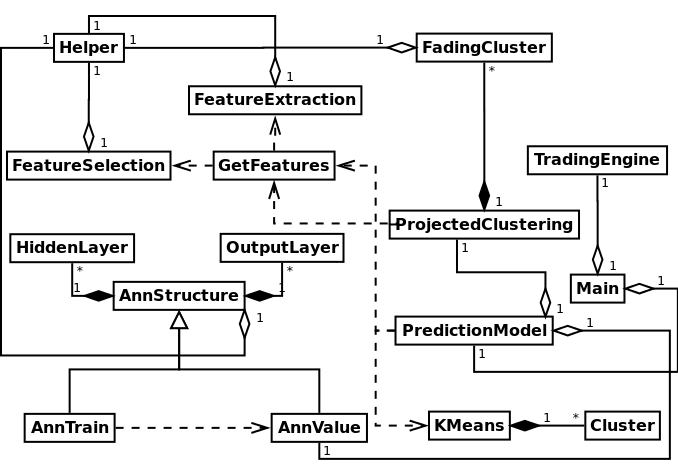
\includegraphics[scale = 0.5]{pictures/projectClass.png}
\caption{Class Diagram}
\label{fig:class_diag}
\end{figure}

We have several classes in our model. Here we provide short description regarding the role played by each of these classes.

\begin{enumerate}
\item \textit{FeatureExtraction}

This class is used to extract the features from the news document. The different function in this class are for extracting the different kinds of features from the news document. It saves the frequency distribution of features in the document using $FreqDist$  from $nltk.probability$. The $Helper$ class is used to save all the features extracted to a file. 

\item \textit{FeatureSelection}

This class is used to select the most representative features which we extracted earlier using the $FeatureExtraction$ class. It contains the different feature selection methods which are used to select the features from the features extracted. 

\item \textit{GetFeatures}

This class uses instances of the \textit{FeatureExtration} and \textit{FatureSelection} to extract features and select from relevant features from them. The document vectors are finally created by the $featureRepresentation$ function. 

\item \textit{HiddenLayer}

This class pertains to the ANN module and is used to define the nodes in the Hidden Layer of the ANN. All functions regarding the hidden layer like calculating output, error and weight updates at each node are carried out by the functions of this class. 

\item \textit{OutputLayer}

This class is used to define the nodes in the Output Layer of the ANN. Te functions of this class also carry out the operations as done by the \textit{HiddenLayer} class functions. 

\item \textit{AnnStructure}

This class is used to define the structure of the ANN network. The network is made up of objects from the \textit{HiddenLayer} and \textit{OutputLayer} classes. So, a composition relation exists with them. 

\item \textit{AnnTrain}

This class is used to train the ANN network. It inherits the network structure from the \textit{AnnStruture} class. The training data set is prepared by normalization according to the activation function used. The network is then trained for minimum error as stated in section-\ref{subsec:training}. The minimum errors obtained are saved for future use. 
\newpage
\item \textit{AnnValue}

This class is used to obtain the results for a particular input vector from the ANN. It inherits the network structure from \textit{AnnStructure}. The minimum error weights which we obtained during training phase is loaded into the network and result outputs are obtained for input vectors.

\item \textit{Cluster}

This class is used to define the structure of a normal cluster. It stores information like cluster number and points in the cluster. 

\item \textit{KMeans}

This class uses the K-means clustering method to form the initial cluster. It contains methods to get the data points. form clusters, calculate centroids, etc. 

\item \textit{FadingCluster}

This class is used to define the structure of the fading clusters and also define the different functions on these clusters like changing the feature space of the clusters, adding new data points to them, finding their limiting radius. 

\item \textit{ProjectedClustering}

This class does the projected clustering on the points in the high dimensional space. It is composed of the $FadingCluster$ class since it works with fading clusters. It uses the $Kmeans$ class to form the initial clusters using the K-means method. 

\item \textit{PredictionModel}

This class is used to carry out the prediction of the index values. It uses the \textit{ProjectedClustering} class to carry out the clustering of the new data point and it uses the \textit{AnnValue} class to predict the index value according to the changes in the various financial parameters and the sentiment of the news which is given by the \textit{ProjectedClustering} class. The predicted values are stored in a file are analyzed and plotted using R language. 

\item \textit{TradingEngine}

This class does the mock trading of stocks in the stock market according to the prediction values. The return value after the stocks are traded is returned. 

\item \textit{Main}

This class is the main class which controls the other classes. The \textit{PredictionModel} and \textit{TradingEngine} are called from this class for the prediction of the values and trading of stocks according to the predicted values. This helps us run the program. 

\item \textit{Helper}

This class contains many functions which help us with simple tasks. It mainly provides the other important classes support. 

\end{enumerate}

\chapter{Experiment and Results}
In this chapter we discuss the different experiments carried out and the results generated by them. Firstly we give the experiment with the ANN changing the various parameters to get the minimum error weight. After that a simulated trading is done to compare results with \cite{Hagenau:2013}. 

\section{Artificial Neural Network training}
The different parameters which we change in the ANN are - number of hidden units used, the learning rate and according to the different activation functions as mentioned in \ref{subsec:activation}.

The normalized errors generated are presented in table-\ref{tab:error}. In the table $\lambda$ is the learning rate and $h$ denotes the number of hidden used in the ANN network. 


\begin{table}[ht]
\centering
\caption{ANN normalized error}
\label{tab:error}

\vspace{15pt}
\begin{tabular}{|l|l|l|l|l|l|l|}
\hline
\multirow{2}{*}{Activation Function} & \multicolumn{3}{c|}{$\lambda$ = 0.5}                                                      & \multicolumn{3}{c|}{$\lambda$ = 0.05}                                                  \\ \cline{2-7} 
                  & \multicolumn{1}{c|}{$h$ = 3} & \multicolumn{1}{c|}{$h$ =2} & \multicolumn{1}{c|}{$h$=1} & \multicolumn{1}{c|}{$h$=3} & \multicolumn{1}{c|}{$h$=2} & \multicolumn{1}{c|}{$h$=1} \\ \hline
Log Sigmoid       & 0.30865                    & 0.30154                   & 0.28158                  & 0.28199                  & 0.2815                   & 0.28136                  \\ \hline
Bipolar Sigmoid   & 18.428                     & 18.42799                  & 18.42799                 & 18.42802                 & 18.42799                 & 18.42799                 \\ \hline
Tan Hyperbolic    & 18.42128                   & 18.42799                  & 18.42712                 & 18.42794                 & 18.42783                 & 18.42807                 \\ \hline
\end{tabular}
\end{table}

From the table-\ref{tab:error} we can see that the sigmoid activation function is the best for our data since it gives the least error. The number of hidden units taken is 1. 

The change in error with the training iterations for the least error configuration as found out is given in figure-\ref{fig:error_plot}.

\begin{figure}[htbp]
\centering
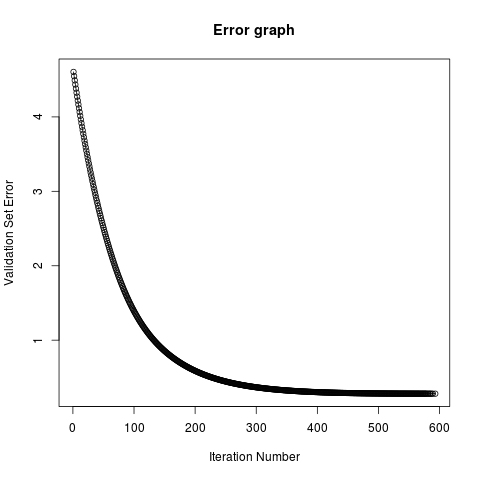
\includegraphics[scale = 0.6]{pictures/errorPlot.png}
\caption{Change in Error over iteration}
\label{fig:error_plot}
\end{figure}

The final structure for our network is 5-1-1 (5 input nodes, 1 hidden node, 1 output node).

\section{BSE Sensex Prediction}

We run our prediction model on 35 days of BSE stock market data and news collected using our \textit{DataCollector} module as described in section-\ref{subsec:data_collection}. The BSE sensex index values are predicted using our prediction model. For each day our model is pre-configured according to the previous day to the trading. We already have an Artificial Neural Network trained according to one month data. 

The different parameters used for our model are given in table-\ref{tab:parameter}. The Initial number of clusters determine the number of clusters to form using kmeans as a part of the initial fading clusters preparation as described in section-\ref{sec:initial_fc}. The Decay Rate ($\lambda$) is a parameter for the Fading Cluster as described in section-\ref{sec:fading}. The Dimensionality ($l$) and Spread Radius Factor ($\tau$) are related to the Projected Clustering (\ref{sec:proj_clustering}).

\begin{table}[h]
\centering
\caption{Parameter Values}
\label{tab:parameter}
\vspace{15pt}
\begin{tabular}{|l|l|l|l|}
\hline
Initial Number of Clusters & Dimensionality ($l$)         & Decay Rate ($\lambda$)               & Spread Radius Factor ($\tau$)     \\ \hline
\multicolumn{1}{|r|}{7}    & \multicolumn{1}{r|}{5} & \multicolumn{1}{r|}{0.3} & \multicolumn{1}{r|}{0.5} \\ \hline
\end{tabular}
\end{table}


A sample prediction plot which we generate from our model is shown in figure-\ref{fig:error_plot}. For each of the 35 days we generate a graph similar to this showing the predicted and actual index value plot with respect to time.

\begin{figure}[htbp]
\centering
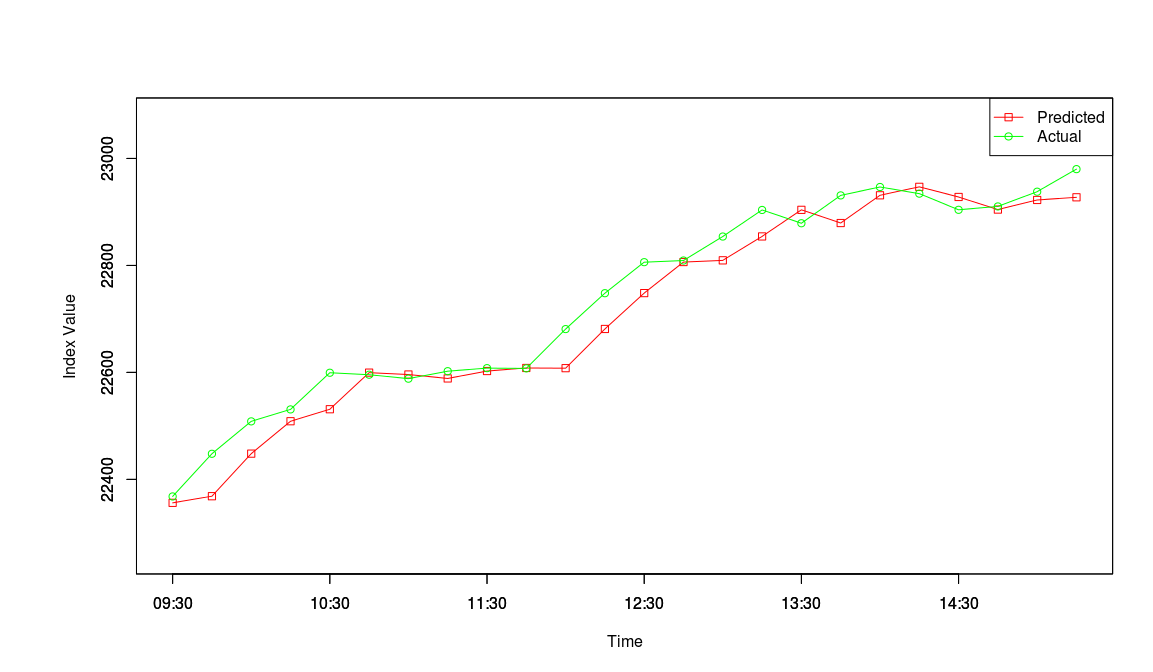
\includegraphics[scale = 0.4]{pictures/predictionResult.png}
\caption{Prediction plot for 9-5-2014 as generated by our model}
\label{fig:error_plot}
\end{figure}

In order to determine the prediction accuracy of our model we use 2 metrics. For the 35 day trading data we find out our model accuracy using these metrics. We define next the two evaluation metrics in detail.
\newpage
The two evaluation metrics used are -

\begin{enumerate}
\item \textbf{Normalized Mean Square Error (NMSE)}

The Normalized Mean Square Error is used to predict the accuracy of our index prediction. It is calculated as - 
\begin{equation}
NMSE = \frac{\sum_{t=1}^{N} (O_t - P_t)^2}{\sum_{t=1}^N (O_t - \bar{O_t})^2}
\end{equation}

where, $t$=[1,N] are the time series points on which values are predicted. For BSE, trading on the BOLT System is conducted from Monday to Friday between 9:15 a.m. and 3:30 p.m. normally \cite{bse_trade}. So, the $t$ value changes in this period of time on those days. $O_t$ and $P_t$ are the Original Value and the Predicted Value at time $t$ respectively. $\bar{O_t}$ is the mean of the original values. This gives us the difference between our prediction results.
\newpage
\item \textbf{Sign Correctness Percentage (SCP)}

This is used to evaluate the performance of the direction prediction. The number of times the model can predict the direction in which the market is about to turn. It is calculated as -
\begin{equation}
SCP = \frac{\{ Sign(P_t) = Sign(O_t) | t = 1,2,...,N\}}{N} \times 100
\end{equation}
\end{enumerate}

The table-\ref{tab:performance} gives the result obtained by running our method on the 35 day stock data collected by us spread over a 10 week span. We give the average NMSE and SCP values of each week trading. 

\begin{table}[ht]
\centering
\caption{NMSE and SCP for 35 days trading}
\label{tab:performance}
\vspace{15pt}
\begin{tabular}{|l|r|r|r|r|r|r|r|r|r|r|r|r|r|r|}
\hline
Week \# & 1 & 2 & 3 & 4 & 5 & 6 & 7 & 8 & 9 & 10 & \textit{Average} \\ \hline
NMSE  & 0.46 & 0.33 & 1.2 & 0.55 & 0.88 & 0.12 & 0.12 & 0.82 & 0.43 & 0.7 & 0.56 \\ \hline
SCP  & 56.43 & 41.67 & 52.78 & 50 & 48.27 & 54.17 & 54.17 & 54.17 & 48.96 & 52.08 & 51.27 \\ \hline
\end{tabular}
\end{table}

\section{Trading Engine}
A trading engine is used to simulate trading in stock market according to our predictions and the return value for trade in the stock market is found out. 

In a highly liquidated market, the 2 main trading strategies used for stocks are - 
\begin{enumerate}
\item Buying of rising stocks, where the stocks are bought at the current value and later sold at a higher value for profit.
\item Short selling of Stocks, stocks which are not currently owned by a trader and will be bought later from the open market at a lower price than current price, thus resulting a profit.
\end{enumerate}

We follow the popular Lavrenko's trading strategy as introduced in \cite{lavrenko2000language}. According to the trading strategy, whenever we see a \textit{positive} trend in the market Rs.10,000 worth of stocks is bought. The trader holds the stocks for 1 hour and then sells it. If during the 1 hour if a profit of 1\% can be done then the stocks are sold immediately. If the trend is \textit{negative} Rs. 10,000 worth of stocks is short-selled. Again after 1 hour time or if 1\% lower price is conceived then the stocks are bought back. At the end of 1 hour the stocks are traded even if loss has to be faced by the trader. Assumptions taken are that the stock transaction costs are zero. 


We do trading on the stocks of \textit{Tata Steel} traded in BSE as \textbf{BOM:500470} in the steel sector. We compare our trading return with those of \cite{Hagenau:2013} in table-\ref{tab:return} and show the comparison of  trade return with similar trading parameters in figure-\ref{fig:trade} . 

\begin{figure}[htbp]
\centering
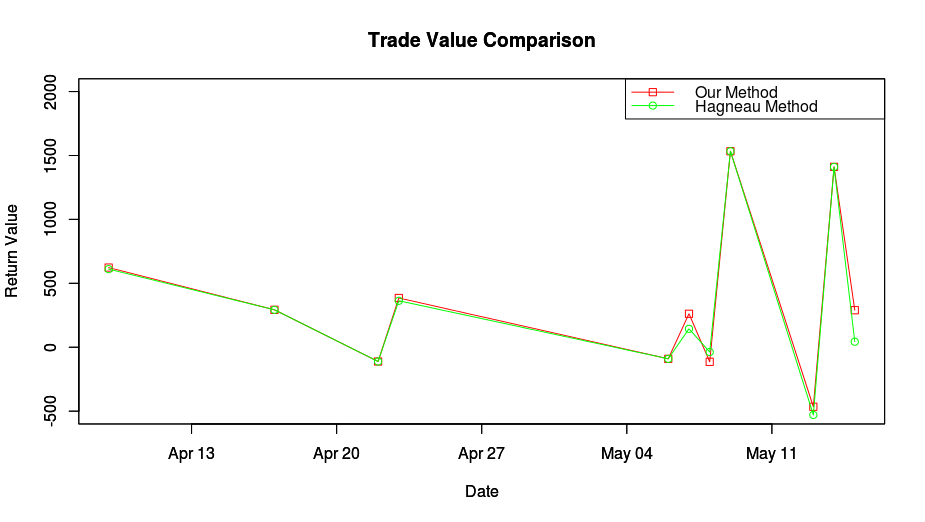
\includegraphics[scale = 0.5]{pictures/tradeReturn.png}
\caption{Stock Simulated Trade Return}
\label{fig:trade}
\end{figure}

Our method shows almost similar in most cases and in some cases better trading returns for the simulated trading as shown in figure-\ref{fig:trade} rather than the one used in \cite{Hagenau:2013}. This shows how our model is more useful for stock trading and gives better trade return. 

\begin{table}[htbp]
\centering
\caption{Trade Percentage Return}
\label{tab:return}
\vspace{15pt}
\begin{tabular}{|c|c|}
\hline
Our Method                   & Hagneau et al. \cite{Hagenau:2013}              \\ \hline
\multicolumn{1}{|r|}{3.65\%} & \multicolumn{1}{r|}{3.3\%} \\ \hline
\end{tabular}
\end{table}

\chapter{Summary and Conclusion}
In summary, our research shows that due to the changing nature of news documents a static feature space is not a good choice, and dynamic feature spaces give better results. We have designed a prediction model for the forecasting of the trading index, and we develop a trading system according to the index prediction. 

A dynamic lossless homogeneous feature space change conversion method is designed. This changes the feature space of the clustering model every time. Features are extracted according to the importance of the word in the current news items. 

The forecasting system uses projected clustering in order to overcome the \textit{Curse of Dimensionality}. The Projected clustering is used for classification of the news documents, which will help predict the trend of the stock market in the next time frame. The projected clustering uses fading cluster structures which help define the way, importance of old news gets reduced over time.

Finally with the use of an Artificial Neural Network we predict the BSE S\&P 500 Sensex index value. The change in the Index value is used to predict the trend in the market and stocks are traded according to these trends. We compare our method with the existing research in \cite{Hagenau:2013}. Our simulated trading system shows much better percentage return results than the existing method.

The method designed in this work can be further investigated in the following ways- 
\begin{enumerate}
\item To capture the concept drift, we have used projected clustering with dynamic feature space. Ensemble Classifiers is also a promising way to capture concept drifts in data streams. Our method can be used with this to see the nature of the change.

\item Our method uses all kinds of news to predict trends. However when we are predicting a particular stock, a model to track the individual sector trends can also be used alongside for better predicting trends relevant to a particular stock.
\end{enumerate}

\titlespacing*{\chapter}{0pt}{10mm}{10mm}
\setlength{\parskip}{\baselineskip}
\bibliographystyle{plain}
\bibliography{references.bib}{}

\chapter*{Acknowledgement}
\thispagestyle{empty}
This project has given me enormous learning opportunities, providing a lot of satisfaction working on it. It has been a nice journey throughout.

I would like to thank my guide, Prof. S. G. Sanjeevi for providing his support and guidance along the way.

I would also like to thank my friends in National Institute of Technology, Warangal who have been like a family for me these past 2 years and always provided moral and technical support in times of need. Special thanks goes out to Sohom Majumdar for helping me out in many ways, specially to become more LaTex savvy.

I would also like to thank my sister and parents who provided me with this opportunity to be here, messing with computer science at higher levels. Thank you for your support throughout. 
\flushright{- Saurav Das}
\end{document}
